%!TEX root = ../luanvan.tex
\chapter{Xây dựng hệ thống}
\section{Tổng quan giải pháp}
Hệ thống quản lý VBCC sử dụng công nghệ blockchain có các chức năng: cấp, quản lý và xác minh VBCC một cách an toàn, bảo mật. Giải pháp được thử nghiệm với nền tảng kỹ thuật số của IBM Blockchain Flatform, Hyperledger Fabric. VBCC có thể được xác thực với tùy chọn hạn chế tiết lộ thông tin và không cần sự can thiệp từ tổ chức cấp chứng chỉ (Trường/Trung tâm).

\begin{figure}[htbp]
\centering
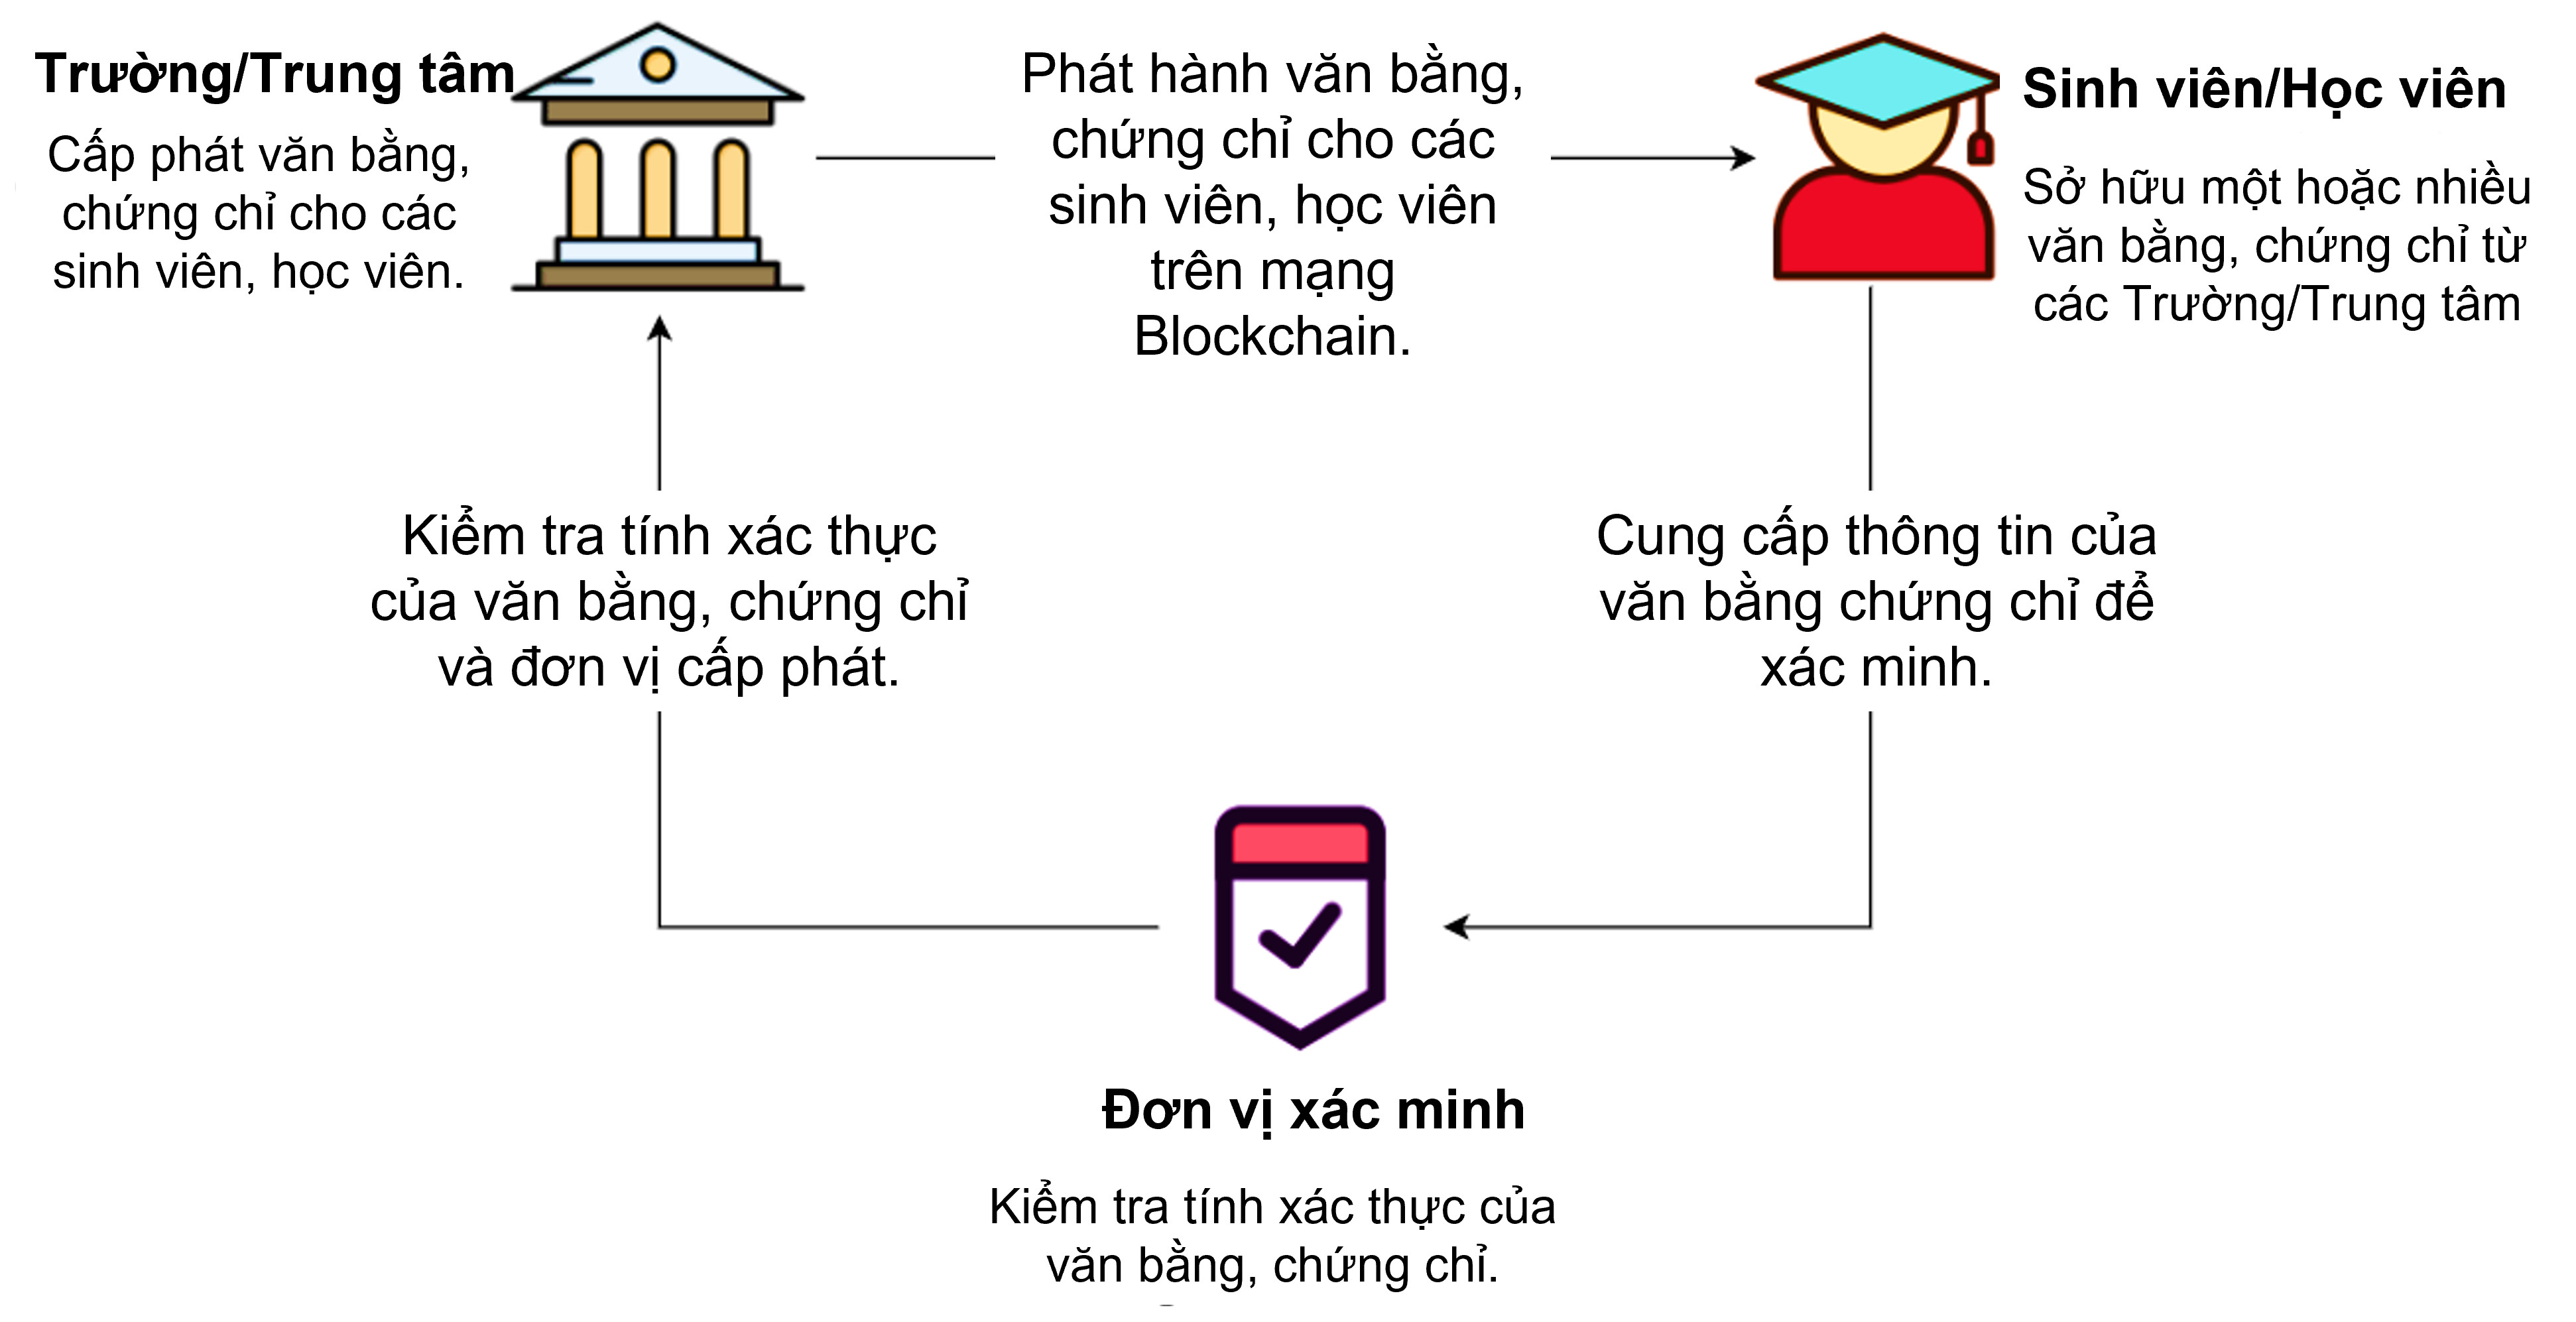
\includegraphics[width=.9\linewidth]{img/vbcc.jpg}
\caption{Sơ đồ tổng quan giải pháp}
\label{fig:vbcc}

\end{figure}
Những chức năng chính của hệ thống được mô tả như hình \ref{fig:vbcc} bao gồm:
\begin{itemize}
\item Trường/Trung tâm: ký số và cấp VBCC.
\item Sinh viên: xem và chia sẻ VBCC.
\item Đơn vị xác minh: kiểm tra tính xác thực của các VBCC được chia sẻ.
\end{itemize}


\section{Kiến trúc phần mềm}
Kiến trúc phần mềm được mô tả như hình \ref{fig:vbcc_phanmem} bao gồm các thành phần:
\begin{figure}[htbp]
\centering
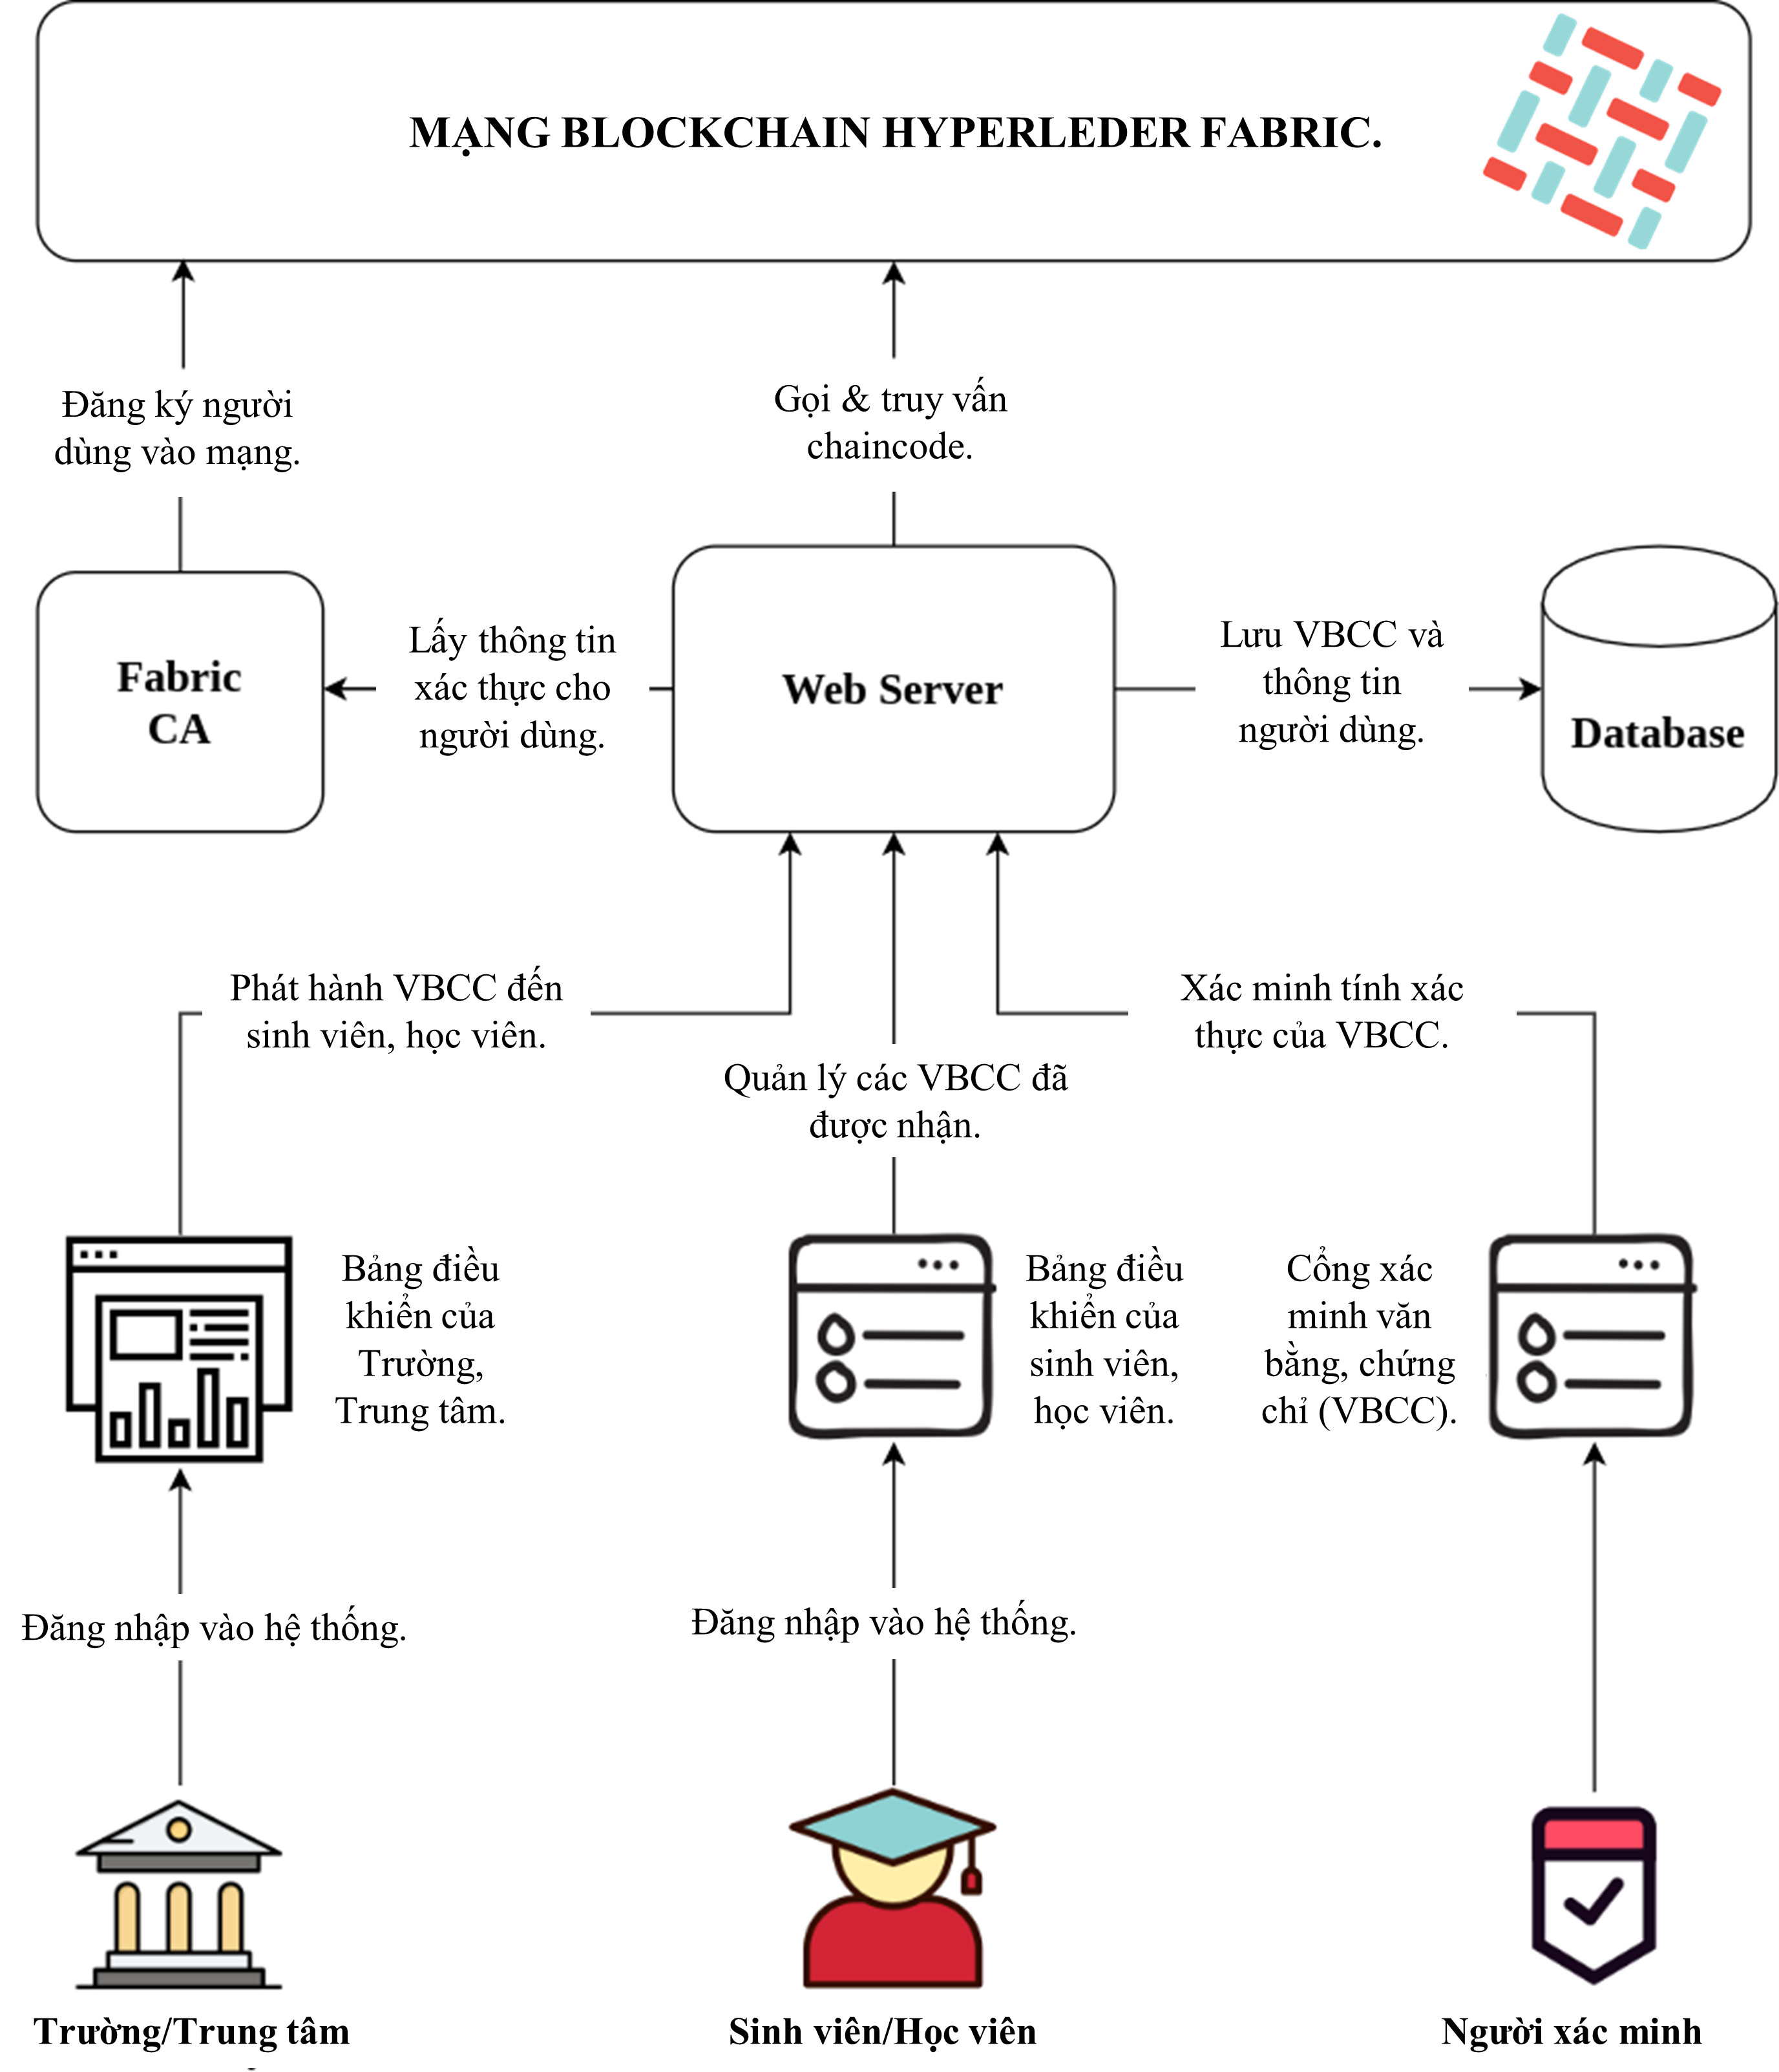
\includegraphics[width=.9\linewidth]{img/vbcc_phanmem.jpg}
\caption{Sơ đồ kiến trúc phần mềm}
\label{fig:vbcc_phanmem}
\end{figure}
\begin{enumerate}
\item Mạng Blockchain Hyperledger Fabric: IBM Blockchain Flatform và Docker container hỗ trợ xây dựng mạng blockchain Fabric, thực thi các hợp đồng thông minh (ngôn ngữ Javascript).
\item Fabric CA: được dùng để đăng ký và xác thực các thành phần trong mạng.
\item Webserver: sử dụng Node.js cung cấp giao diện Backend của ứng dụng web, kết hợp sử dụng Nodejs Express.
\item Cơ sở dữ liệu MongoDB: lưu trữ dữ liệu người dùng và chứng chỉ.
\item Giao diện Front-end của ứng dụng web: dùng các thư viện Bootstrap, jQuery.
\end{enumerate}

\section{Các thành phần tham gia}
Các thành phần tham gia của hệ thống bao gồm: (1) Trường, Trung tâm, (2) Sinh viên (học viên) và (3) Bên xác minh chứng chỉ (Ví dụ: nhà tuyển dụng). Mỗi thành phần sẽ có các hành động như sau:

\emph{Trường, trung tâm}

\begin{itemize}
\item Đăng ký tài khoản.
\item Đăng nhập tài khoản.
\item Cấp VBCC có xác nhận chứng thực và ký số VBCC.
\item Xem VBCC đã cấp.
\end{itemize}

\emph{Sinh viên, học viên}

\begin{itemize}
\item Đăng ký tài khoản.
\item Đăng nhập tài khoản.
\item Xem VBCC đã nhận.
\item Chia sẻ thông tin VBCC.
\item Tiết lộ thông tin VBCC có chọn lọc nhằm hạn chế lộ thông tin.
\end{itemize}

\emph{Bên xác minh chứng chỉ}

\begin{itemize}
\item Xác minh tính xác thực của VBCC với nền tảng blockchain.
\end{itemize}


